{
     \lstset{
        numbers=none,
        numberstyle=\scriptsize,
        language=[LaTeX]TeX,
        commentstyle=\color{white},
        keywordstyle=\color{blue}
 }
%   这是为了插入LaTeX代码

%  正文章节从下面开始
\chapter{模板使用}
\songti\xiaosi
\begin{spacing}{1.5}

本项目为非官方的南京理工大学本科生毕业论文(经管、文科类)\LaTeX 模板,考虑目前没人制作本科生毕设模板,小白一枚的本人自告奋勇地制作了该模板,基本上符合2017年南京理工本科生毕业论文官方模板word板格式,如有问题之处欢迎大家向我提出。

此外本人在此声明:目前只有我自己使用此模板完成过毕业设计(注:我用的理工类),任何人使用本模板进行该模板排版均属于自愿行为,如发生任何问题,本人概不负责。

\section{图片使用}
为了方便于管理,所有的图片均放在figure文件下。在输入图片名称时,需要在前面添加一个相当于路径的语句“figure//”,以下文本框中给出一个图片插入的例子。在某些情况下,如果不想让图片浮动把\fbox{[htb]}选项改成\fbox{[H]},H为强制禁止浮动,但会拉宽段间距和公式与正文之间距离,结合自己需求进行调整。这里已经把图片标题的格式和前后间距都已经设置,可以直接使用“$\setminus$caption”即可。

\begin{lstlisting}
\begin{figure}[htb]
  \centering
  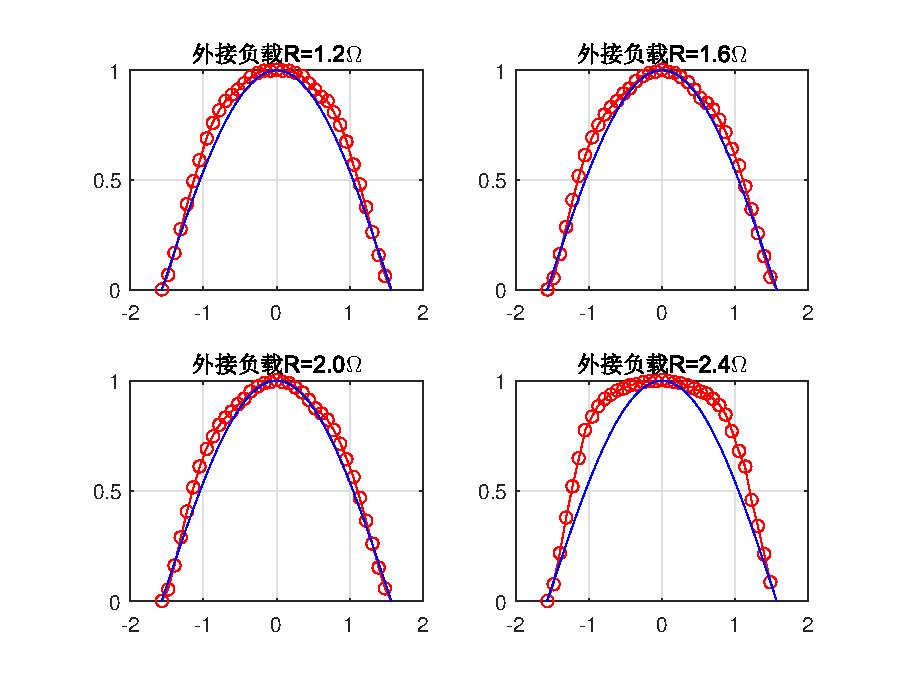
\includegraphics[width=0.65\textwidth]{figure//fig_calculate}
  \caption{SampleFigure}\label{samplefigure}
\end{figure}

\end{lstlisting}

下图\ref{samplefigure}上面程序得到图片效果。

\begin{figure}[htbp]
  \centering
  % Requires \usepackage{graphicx}
  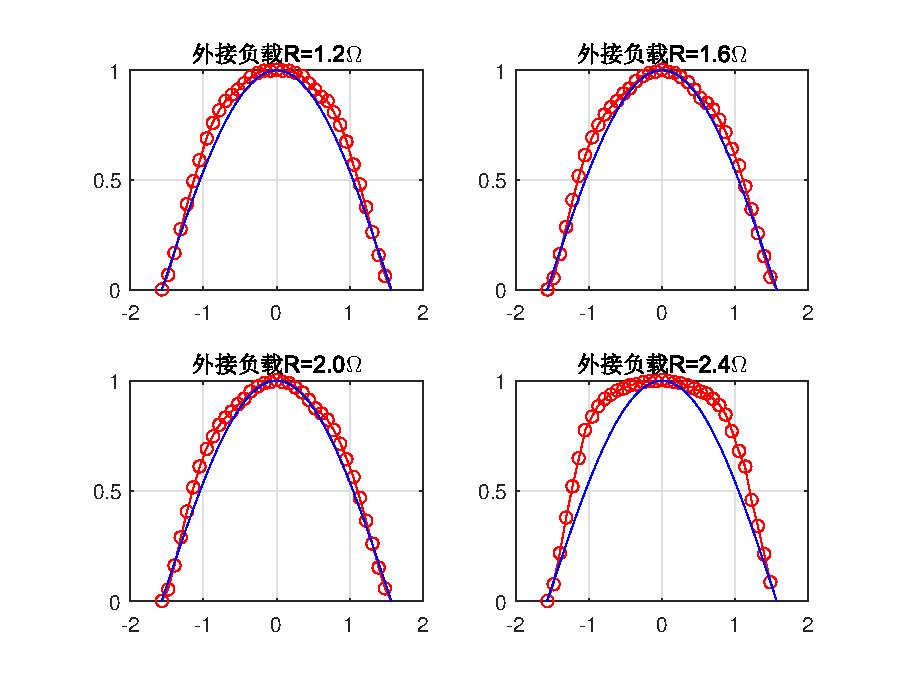
\includegraphics[width=0.65\textwidth]{figure//fig_calculate}
  \caption{SampleFigure}\label{samplefigure}
\end{figure}

\section{表格使用}
由于学校要求三线表格,自己在制作时需要注意该点,表格中的文字应该为五号宋体,结合两点要求,文本框中给出一个表格的范例。为了区分和图片的标题命名,在使用表格时使用“$\setminus$topcaption”,表格标题的格式和前后间距都已经设置。

\begin{lstlisting}
{\zihao{5}\songti
\begin{table}[htb]
\begin{center}
\topcaption{SampleTable}\label{sampeltable}
\begin{tabular}{m{3cm} m{2cm} m{2cm} m{2cm}}
  \hline
  Project & A & B & C\\
  \hline
  ProjectOne   & a1 & b1 & c1 \\
  ProjectTwo   & a2 & b2 & c2 \\
  ProjectThree & a3 & b3 & c3 \\
  ProjectFour  & a4 & b4 & c4 \\
  ProjectFive  & a5 & b5 & c5 \\
  \hline
\end{tabular}
\end{center}
\end{table}}
\end{lstlisting}

下表\ref{sampeltable}是一个表格示例。

{\wuhao\songti
\begin{table}[htb]
\begin{center}
\topcaption{SampleTable}\label{sampeltable}
\begin{tabular}{m{3cm} m{2cm} m{2cm} m{2cm}}
  \hline
  Project & A & B & C\\
  \hline
  ProjectOne& a1 & b1 & c1 \\
  ProjectTwo & a2 & b2 & c2 \\
  ProjectThree & a3 & b3 & c3 \\
  ProjectFour& a4 & b4 & c4 \\
  ProjectFive & a5& b5 & c5 \\
  \hline
\end{tabular}
\end{center}
\end{table}}

考虑到使用该模板大部分是和我一样的小白,这里做一个小提示,毕业设计由于图表都比较多,如果在正文中用到图1.1、表1.1、 式1.1 等词,最好在正文使用\fbox{图$\setminus$ref\{samplefigure\}}、\fbox{表$\setminus$ref\{sampeltable\}}对图表的标号确定。当然前提是figure和table中已经用\fbox{$\setminus$label\{samplefigure\}}、\fbox{$\setminus$label\{sampeltable\}} 进行标记。每个图标和公式的标记应该是唯一的,重复会出现警告。

上述方法是为了避免在写作过程,突然需要前面的图表和公式进行增添或删减,不再需要手动改图标的标号。

\section{公式使用}
对于公式使用\fbox{$\setminus$begin\{equation\}}环境,如果有多行公式可以使用\fbox{$\setminus$begin\{split\}}环境,符号“\&”为各行公式对齐的位置。

如果需要对公式中的字母进行注释,并且注释较多,这里推荐一种方法,可以使用表格的环境,表格为2列,第一列字母靠右,第二列解释靠左,如\fbox{$\setminus$begin\{tabular\}\{r@\{---\}l\}}。 
下面文本框中给出了一个多行公式以及注释的示例。
\begin{lstlisting}
\begin{equation}\label{SampleEquation}
  \begin{split}
  \bm{x_}k&=\bm{\Phi}_{k,k-1}\bm{x}_{k-1}+\bm{\Gamma}_{k-1}\bm{w}_{k-1}\\
  \bm{z}_k&=\bm{H}_k\bm{x}_k+\bm{v}_k
  \end{split}
\end{equation}
\begin{tabular}{r@{---}l}
  $\bm{x}_k$  & The state variable of the $k^{th}$ step;\\
  $\bm{z}_k$  & The observation of the $k^{th}$ step; \\
  $\bm{\Phi}_{k,k-1}$ & The transition matrix of the $(k-1)^{th}$ to $k^{th}$ step; \\
  $\bm{\Gamma}_{k-1}$  & The measurement noise driving matrix of the $k^{th}$ step; \\
  $\bm{H}_k$  & The measurement matrix of the $k^{th}$ step;\\
  $\bm{w}_{k-1}$ & The systematic noise of the $(k-1)^{th}$ step ,$\bm{w}_{k-1}\sim N(0,\bm{Q}_{k-1})$;\\
  $\bm{v}_k$ & The measurement noise of the $k^{th}$ step,$\bm{v_k}\sim N(0,\bm{R}_k)$.
\end{tabular}
\end{lstlisting}

下式\ref{sampeltable}和注释为上面程序的效果,数学符号可以自行百度,或者在这\url{http://www.mohu.org/info/symbols/symbols.htm}上面寻找,几乎包含了基本上要用的数学符号。
\begin{equation}\label{SampleEquation}
  \begin{split}
  \bm{x_}k&=\bm{\Phi}_{k,k-1}\bm{x}_{k-1}+\bm{\Gamma}_{k-1}\bm{w}_{k-1}\\
  \bm{z}_k&=\bm{H}_k\bm{x}_k+\bm{v}_k
  \end{split}
\end{equation}
式中:

\begin{tabular}{r@{---}l}
  $\bm{x}_k$  & The state variable of the $k^{th}$ step;\\
  $\bm{z}_k$  & The observation of the $k^{th}$ step; \\
  $\bm{\Phi}_{k,k-1}$ & The transition matrix of the $(k-1)^{th}$ to $k^{th}$ step; \\
  $\bm{\Gamma}_{k-1}$  & The measurement noise driving matrix of the $k^{th}$ step; \\
  $\bm{H}_k$  & The measurement matrix of the $k^{th}$ step;\\
  $\bm{w}_{k-1}$ & The systematic noise of the $(k-1)^{th}$ step ,$\bm{w}_{k-1}\sim N(0,\bm{Q}_{k-1})$;\\
  $\bm{v}_k$ & The measurement noise of the $k^{th}$ step,$\bm{v_k}\sim N(0,\bm{R}_k)$.
\end{tabular}

\section{参考书籍}
参考文献在ThesisReference中\fbox{$\setminus$begin\{thebibliography\}}环境中进行填写,具体格式规范查阅参考文献标注国家标准GB/T~7714——2015。

模板参考文献使用下面文本框中方法,该方法比较业余,不便于大量参考文献的管理,并且需要手动输入书目信息。专业的方法是使用BibTeX,使用方法自行百度,BibTeX可以在Google scholar、百度学术上直接导入。
\begin{lstlisting}
\begin{thebibliography}
\bibitem author,article, year, vol,
\end{thebibliography}
\end{lstlisting}

正文需要引用文献,使用\fbox{$\setminus$cite\{\}}即可。

\section{代码插入}
考虑到大多数同学的代码应该是MATLAB,在ThesisAppendix文件中将语言设置m语言,可以根据自身需要进行改变。网上的Mcode包编译效果非常不错,这里就直接拿来,做一回拿来主义。

Mcode包效果在附录B MATLAB Code中看到,其能较好地还原MATLAB本身的编程风格。程序代码需放到\fbox{$\setminus$begin\{lstlisting\}}环境中。

\end{spacing}
}